\documentclass[dvipdfmx,autodetect-engine,titlepage]{jsarticle}
\usepackage[dvipdfm]{graphicx}
\usepackage{ascmac}
\usepackage{fancybox}
\usepackage{listings}
\usepackage{plistings}
\usepackage{itembkbx}
\usepackage{amsmath}
\usepackage{url}
\usepackage{graphics}
\usepackage{listings}
\usepackage{here}

\lstset{%
  language={C},
  basicstyle={\small},%
  identifierstyle={\small},%
  commentstyle={\small\itshape\color[rgb]{0,0.5,0}},%
  keywordstyle={\small\bfseries\color[rgb]{0,0,1}},%
  ndkeywordstyle={\small},%
  stringstyle={\small\ttfamily\color[rgb]{1,0,1}},
  frame={tb},
  breaklines=true,
  columns=[l]{fullflexible},%
  numbers=left,%
  xrightmargin=0zw,%
  xleftmargin=3zw,%
  numberstyle={\scriptsize},%
  stepnumber=1,
  numbersep=1zw,%
  lineskip=-0.5ex%
}

\textheight=23cm
\renewcommand{\figurename}{図}
\renewcommand{\tablename}{表}
\newenvironment{code}
{\vspace{0.5zw}\VerbatimEnvironment  \begin{screen} 
\baselineskip=1.0\normalbaselineskip
 \begin{Verbatim}}
{\end{Verbatim}
\baselineskip=\normalbaselineskip
 \end{screen}\vspace{0.5zw}} 

\title{セキュリティ・ネットワーク学実験3(B2)\\
Webアプリケーション脆弱性演習\\
}
\author{2600200087-2\\Oku Wakana\\奥 若菜}
\date{July 9 2022} 

\begin{document}

\maketitle

\section{クロスサイト・スクリプティング}
\subsection{脆弱性の概要および発見演習}
\subsubsection{クロスサイト・スクリプティングの概要}
クロスサイト・スクリプティングの脆弱性とは、不正なスクリプトを何らかの手段でWebページに埋め込むことで、
その不正なスクリプトが被害者のブラウザ上で実行されてしまう脆弱性である。この脆弱性が利用されることで、偽のWebページが表示されたり、Cookieが不正に取得されるといった被害が発生する。\\
\subsubsection{脆弱性の発見手法}
HTMLで出力する時に「\textgreater」を「\&lt;」に置換するなど、特別な意味を持つ文字を、特別な意味を持たない表記文字に置換することをエスケープ処理と言う。
受け取った入力データを、エスケープ処理を行わずに画面に出力している箇所があれば、クロスサイト・スクリプティングの脆弱性となる。\\

\subsubsection{脆弱性の発見演習}
下の図1のより、脆弱性のあるプログラムの名前欄に「'\textgreater "\textgreater \textless hr\textgreater」と入力し、リクエスト送信したところ、出力画面に水平な線が表示された。
また、図2のより、対策が行われているプログラムに同じ入力を行ったところ、入力した文字列がそのまま表示された。\\
\begin{figure}[H]
  \centering
  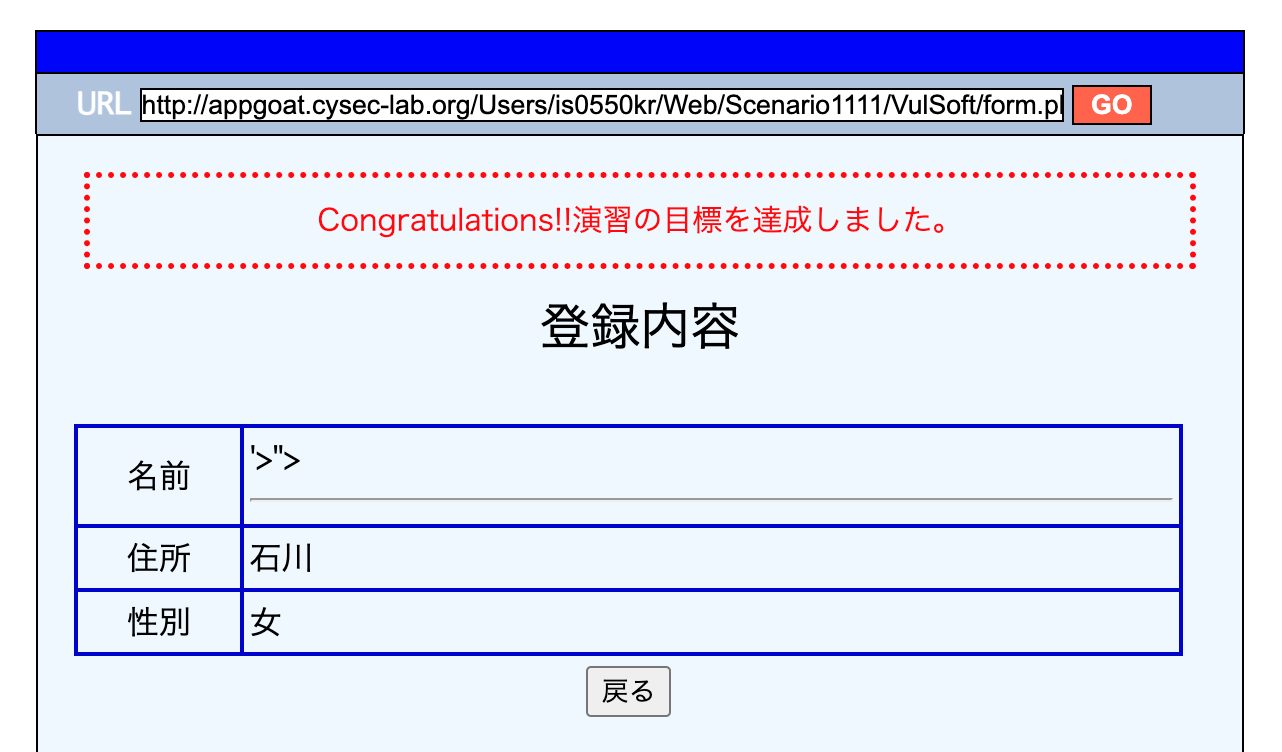
\includegraphics[scale=0.35]{web2.png}
  \caption{脆弱性のあるプログラム}\label{fig:図2}
\end{figure}

\begin{figure}[H]
  \centering
  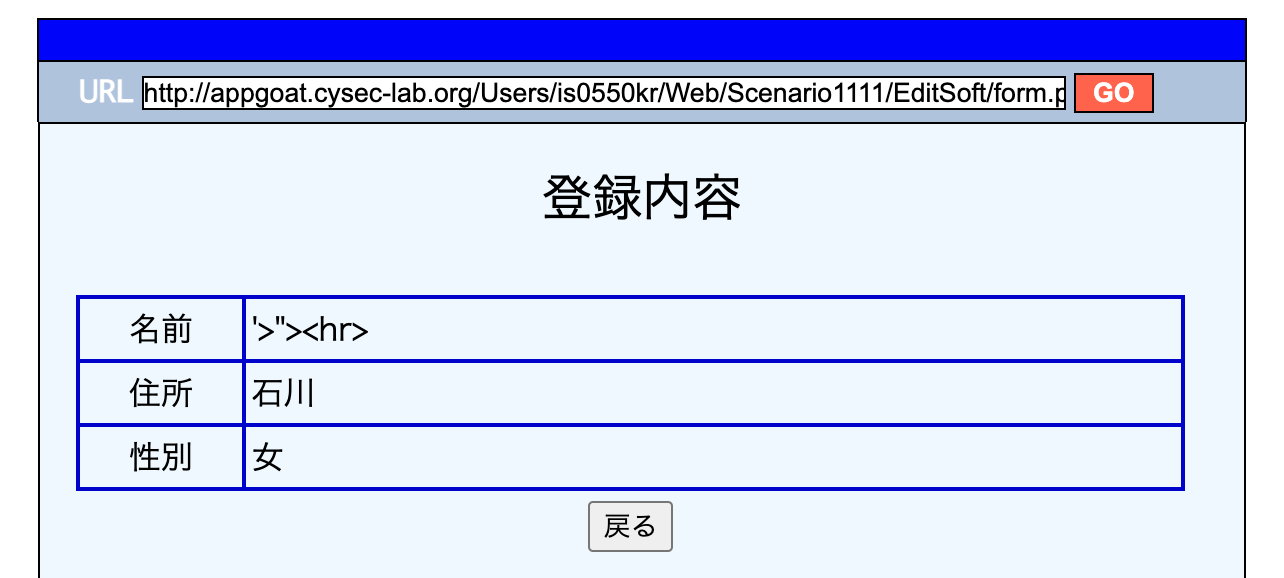
\includegraphics[scale=0.35]{web1.png}
  \caption{対策の行われているプログラム}\label{fig:図1}
\end{figure}

これらのフレーム内のソースコードを示した図3,4より、脆弱性のあるプログラムでは\textless hr\textgreater がタグとして扱われているのに対し、
対策の行われているプログラムでは、全てが文字列として扱われていることが分かる。\\
\begin{figure}[H]
  \centering
  \begin{minipage}[b]{0.45\linewidth}
  \begin{center}
    \fbox{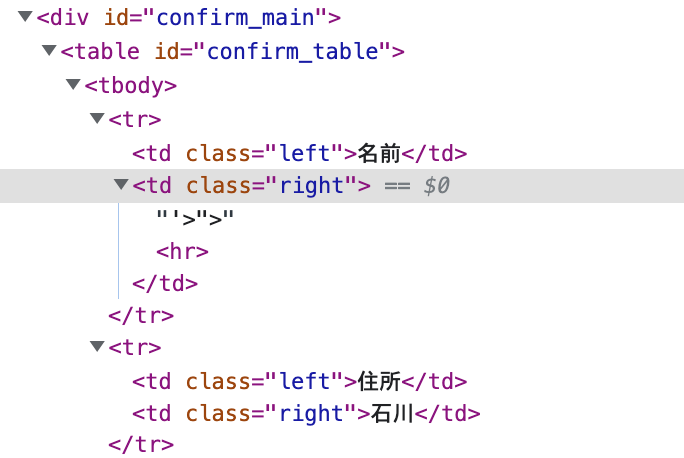
\includegraphics[keepaspectratio,scale=0.5]{web3.png}}
    \end{center}
    \caption{脆弱性のあるプログラム}
  \end{minipage}
  \begin{minipage}[b]{0.45\linewidth}
  \begin{center}
    \fbox{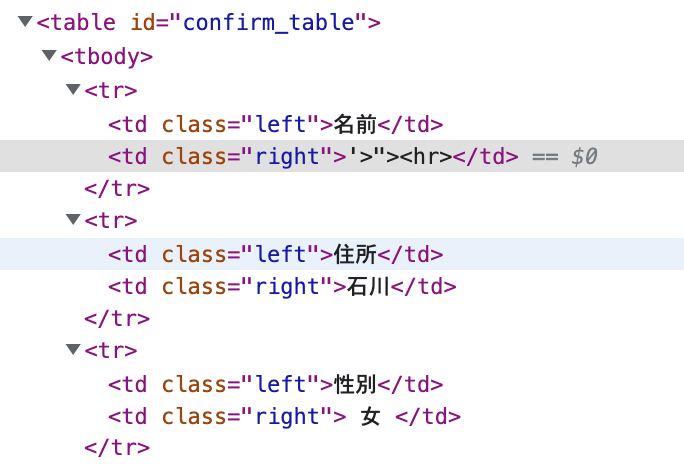
\includegraphics[keepaspectratio,scale=0.5]{web4.png}}
    \end{center}
    \caption{対策の行われているプログラム}
  \end{minipage}
\end{figure}


 \\
\subsection{アンケートページの改ざん(反射型)}
反射型クロスサイト・スクリプティングの脆弱性とは、Webアプリケーションがユーザから受け取った入力データを、そのままの形(実行可能な形)でウェブページの出力に利用してしまう問題である。
アンケートページの名前欄に反射型の脆弱性が発見できたため、名前欄に相当するパラメータである「name」の値にスクリプトを書き込み、作成したURLを名前欄に入力した。\\\\
下の図5,6はそれぞれ実行前と実行後のアンケートページの画面である。リクエストを送信することで、
「*のついている項目は入力必須です。」という注意書きを書き換えることができた。\\
\begin{figure}[H]
  \centering
  \begin{minipage}[b]{0.45\linewidth}
  \begin{center}
    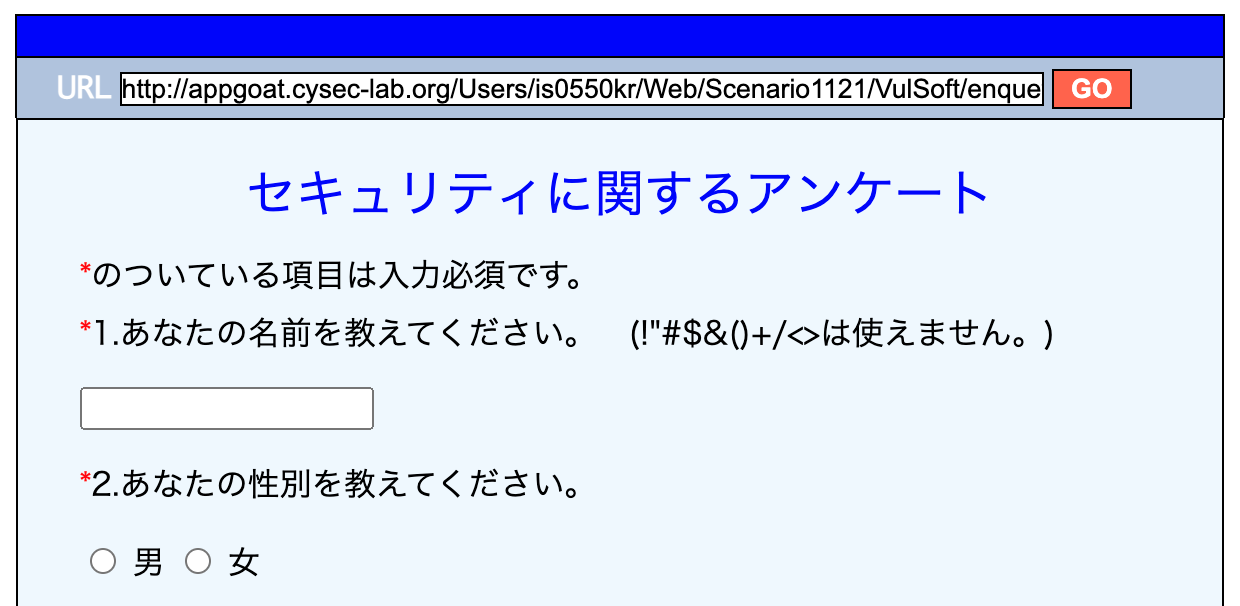
\includegraphics[keepaspectratio,scale=0.33]{web5.png}
    \end{center}
    \caption{実行前の画面}
  \end{minipage}
  \begin{minipage}[b]{0.45\linewidth}
  \begin{center}
    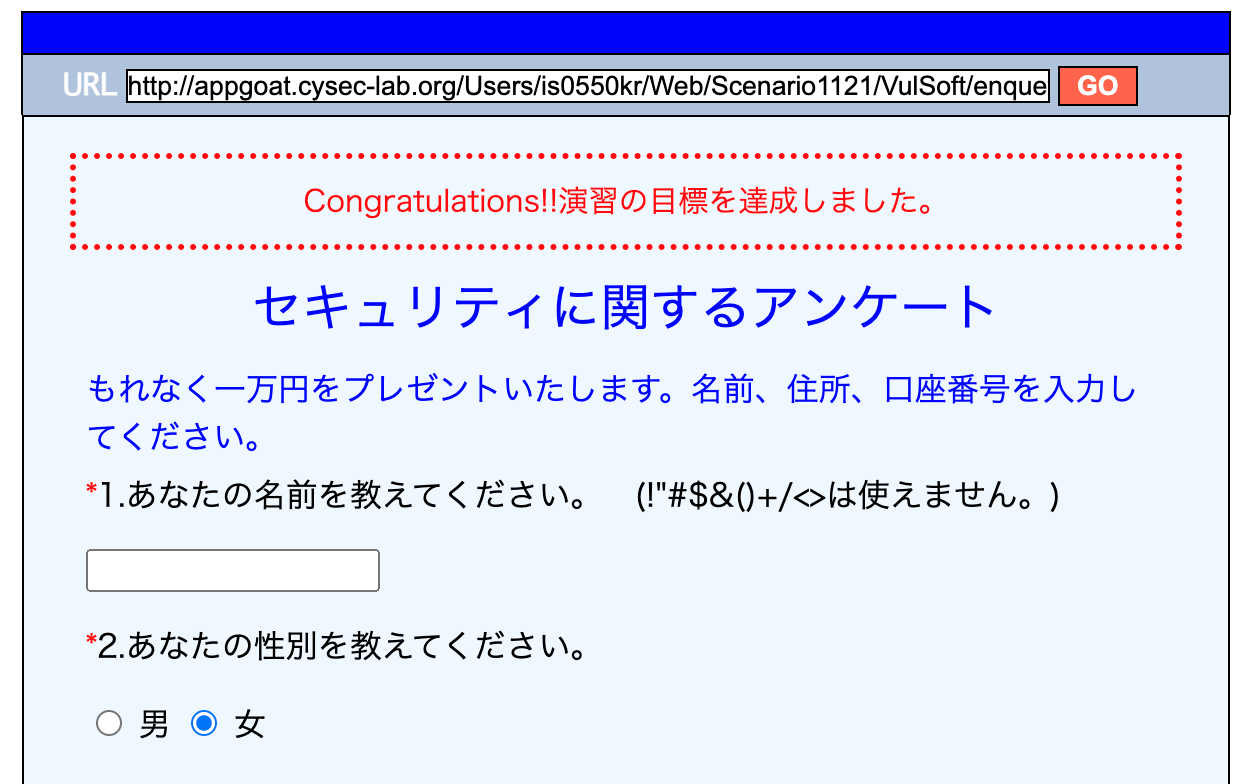
\includegraphics[keepaspectratio,scale=0.3]{web6.png}
    \end{center}
    \caption{実行後の画面}
  \end{minipage}
\end{figure}

 \\\\

\subsubsection{入力情報の漏洩(反射型)}
投稿ボタンをクリックすると、ポップアップダイアログによって送信先を表示するようなアンケートページにおいて、送信先を変更するようなスクリプトを含むURLを作成し、名前欄に見つかった反射型の脆弱性を利用してスクリプトを実行させた。\\\\
下の図7,8はそれぞれ実行前と実行後で、表示されたポップアップをキャプチャしたものである。内容を見ると送信先のURLが書きかわっていることが確認できる。

\begin{figure}[H]
  \centering
  \begin{minipage}[b]{0.45\linewidth}
  \begin{center}
    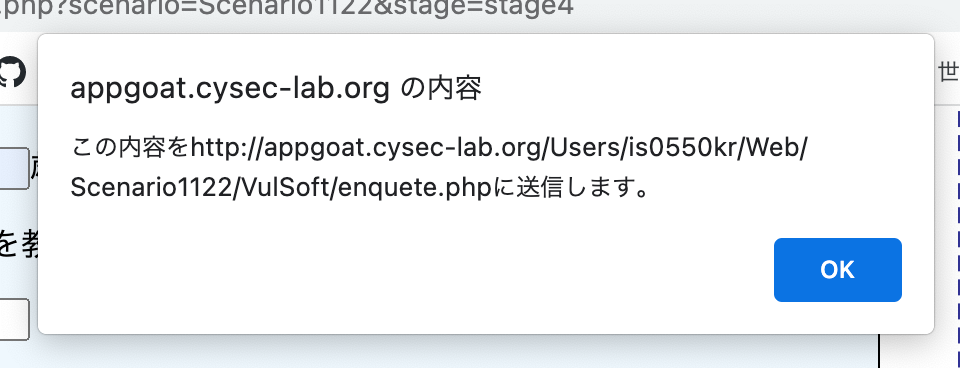
\includegraphics[keepaspectratio,scale=0.4]{web7.png}
    \end{center}
    \caption{実行前の画面}
  \end{minipage}
  \begin{minipage}[b]{0.45\linewidth}
  \begin{center}
    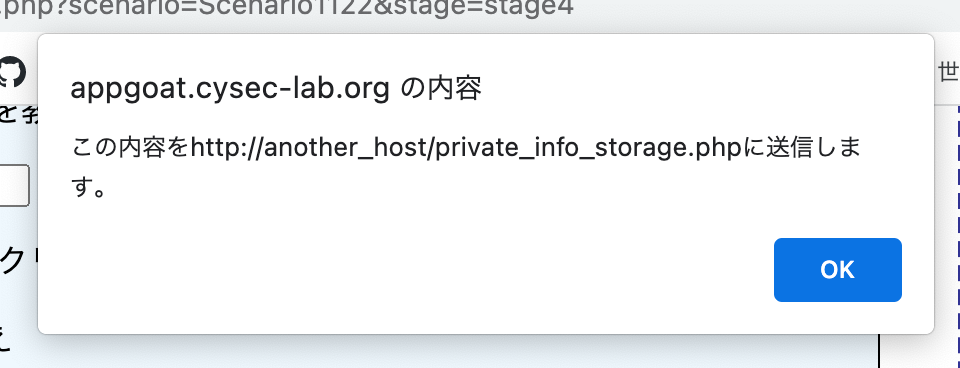
\includegraphics[keepaspectratio,scale=0.4]{web8.png}
    \end{center}
    \caption{実行後の画面}
  \end{minipage}
\end{figure}



\end{document}